\title{Infinite Jest: An Elegant Hairball}
\author{
  Hunter Wapman
  \and
  Brian Lubars
  \and
  Carl Mueller
}
\date{\today}

\documentclass[12pt]{article}
\usepackage[margin=1in]{geometry}
\usepackage{amsmath}
\usepackage{enumitem}
\usepackage{graphicx}
\usepackage{listings}
% \usepackage{physics}
% \usepackage{subfig}
\usepackage{hyperref}
\usepackage{graphicx} % for pdf, bitmapped graphics files
\usepackage{caption}
\usepackage{subcaption}
\usepackage{wrapfig}
\usepackage[font={small}]{caption}


\renewcommand\thesubsection{\alph{subsection}}


\begin{document}
\maketitle

\section*{Introduction}

\subsubsection*{Infinite Jest Book}

\subsubsection*{Why a Network?}

\subsubsection*{Questions..questions that need answering}

\section*{Data Processing}

\subsubsection*{Data Source \& Preprocessing}
To generate a usable text this project utilized an existing `.mobi' file of Infinite Jest. This file was put through a .mobi to HTML conversion to generate an HTML formatted file. This enabled the use of regular expressions to find and parse various text features automatically. However, the abundant HTML annodation prevented the clean usage on Natural Language Processing (NLP) libraries for analyzing text. Thus the HTML text was used to identify where in raw text endnote tags could be placed to identify endnote locations. Similarly, regular expressions were used to indentify where in a raw text version of the text section breaks exist according to the section annotations given by the book Elegant Complexity \cite{carlisle_2007}. The raw text was split on these sections and saved into separate files. Likewise each endnote was saved into a separate file. In each of these files, we removed all special characters that did not seem essential to name entities ("speicial quotes"). As we were utlizing the Python 3.7 standard, all text files were imported as unicode.

\subsubsection*{Named Entitiy Recognition}

A major challenge with Infinite Jest is the abundant use of pseudonyms and aliass from the 200+ characters in the novel. As the desired network would used characters as nodes, identifying named entity and coreference resoluation (but not for pronouns) required an extension hand-engineered approach to correctly indentifying named entities throughout the text. We utilized the Named Entity Recognition (NER) parser of the Python library SpaCy \cite{spacy2} augmented with its own Matcher parser. By running the existing NER model on the text, candidate entities through which manual parsing over these results enabled us to build a Matcher entity file. This enabled Spacy to indentify a large number of the pseudonyms and aliases and their locations within each section of the text.

\subsubsection*{Challenges and Considerations}
One major affront to the Matcher approach is the extensive used of pronoun coreferences. While there are some approaches for coreference resolution at this granularity, most are trained on models not well suited for the very unstructured and informal style of David Foster Wallace. Similarly, the extensive use of dialog presented a challenge in identifying named entities. As such, the use of named entities as nodes, and our methodlogy for identifying where they exist in text, really only enables the generation of a co-mention network. Such a network may only loosly correlated with true latent interaction structure of the book.  


\section*{Network Design}

\subsubsection*{Nodes and Edges}
Network nodes constitute each character identified in the set of found named entities. These were referenced against online resources to ensure proper coverage of the characters in the book. Edges in the book represent a co-mention between two entities in the text. A threshold number of tokens (words) under which the number of tokens between the mention of one entity and another determines if an edge is established. If the edge already exists, the weight is updated. The current entity $i$ is only matched with proceeding entities $j$ within this threshold. Once no match is found, the next available entity is checked for proceeding matches.

The threshold number of tokens is determined by a semi-objective measure of the effect of the threshold length on the average clustering coefficient and the giant component size (see Figure \ref{fig-threshold-size}). The intuition behind the use of these metrics is that we choose the minimum threhold length to produce, at a minimum a large giant component and ample enough clustering.


\begin{figure*}[h]
	\centering
	\begin{subfigure}{0.4\textwidth}
		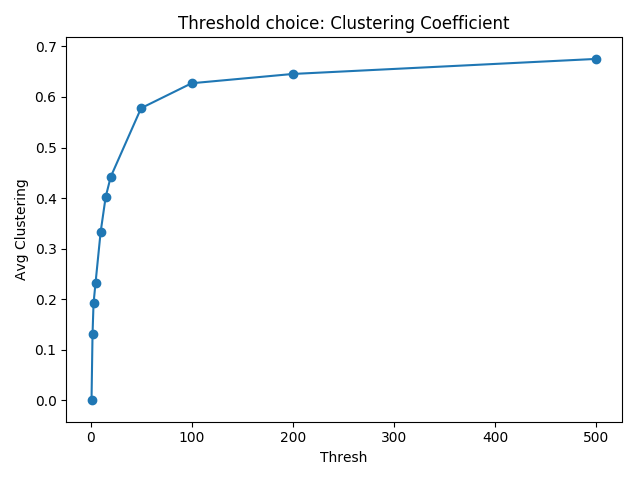
\includegraphics[width=1.\textwidth]{data/plots/thresh_vs_avg_clustering.png}
		\caption{Clustering Coefficient vs. Threshold Size}
	\end{subfigure}
	~
	\begin{subfigure}{0.4\textwidth}
		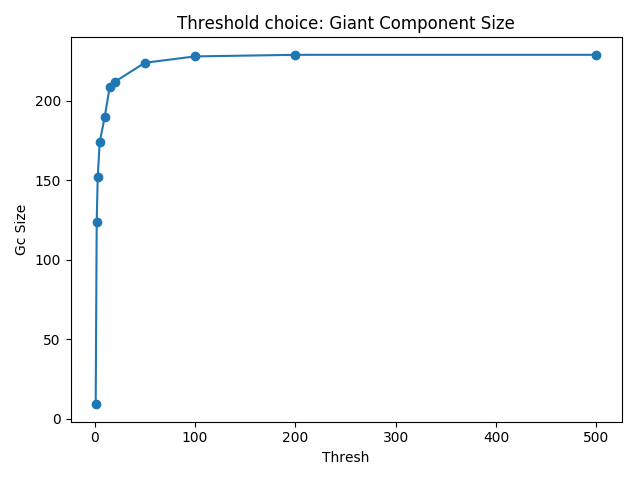
\includegraphics[width=1.\textwidth]{data/plots/thresh_vs_gc_size.png}
		\caption{Giant Component Size vs. Threshold Size}
	\end{subfigure}
	\caption{Comparing threshold size effect on clustering coefficient and giant component size in order to determine the ideal threshold size.}
   	\label{fig-threshold-size}
\end{figure*}


\bibliographystyle{unsrt}
\bibliography{references.bib}
\end{document}
